
%%%%%%%%%%%%%%%%%%%%%%% file typeinst.tex %%%%%%%%%%%%%%%%%%%%%%%%%
%
% This is the LaTeX source for the instructions to authors using
% the LaTeX document class 'llncs.cls' for contributions to
% the Lecture Notes in Computer Sciences series.
% http://www.springer.com/lncs       Springer Heidelberg 2006/05/04
%
% It may be used as a template for your own input - copy it
% to a new file with a new name and use it as the basis
% for your article.
%
% NB: the document class 'llncs' has its own and detailed documentation, see
% ftp://ftp.springer.de/data/pubftp/pub/tex/latex/llncs/latex2e/llncsdoc.pdf
%
%%%%%%%%%%%%%%%%%%%%%%%%%%%%%%%%%%%%%%%%%%%%%%%%%%%%%%%%%%%%%%%%%%%


\documentclass[runningheads,a4paper]{llncs}

\usepackage{amssymb}
\setcounter{tocdepth}{3}
\usepackage{graphicx}
\usepackage{color}

\usepackage{url}
\urldef{\mailsa}\path|{alfred.hofmann, ursula.barth, ingrid.haas, frank.holzwarth,|
\urldef{\mailsb}\path|anna.kramer, leonie.kunz, christine.reiss, nicole.sator,|
\urldef{\mailsc}\path|erika.siebert-cole, peter.strasser, lncs}@springer.com|    
\newcommand{\keywords}[1]{\par\addvspace\baselineskip
\noindent\keywordname\enspace\ignorespaces#1}

\begin{document}

\mainmatter  % start of an individual contribution

% first the title is needed
\title{Inferring Properties of Causal Structure from Student
Essays}

% a short form should be given in case it is too long for the running head
\titlerunning{Inferring Properties of Causal Structure from Student
Essays}

% the name(s) of the author(s) follow(s) next
%
% NB: Chinese authors should write their first names(s) in front of
% their surnames. This ensures that the names appear correctly in
% the running heads and the author index.
%
\author{Simon Hughes\inst{1}%
\thanks{The assessment project described in this article is funded, in part, by the Institute for Education Sciences, U.S. Department of Education (Grant R305G050091 and Grant R305F100007). The opinions expressed are those of the authors and do not represent views of the Institute or the U.S. Department of Education.}%
\and Peter Hastings\inst{1} \and Anne Britt\inst{2}\and \\ Dylan Blaum
\inst{2} \and Patty Wallace\inst{2}}
\authorrunning{Hastings, Hughes, Britt, Blaum, and Wallace}
\institute{DePaul University, Chicago, Illinois
\and
Northern Illinois University, DeKalb, Illinois}

%
% NB: a more complex sample for affiliations and the mapping to the
% corresponding authors can be found in the file "llncs.dem"
% (search for the string "\mainmatter" where a contribution starts).
% "llncs.dem" accompanies the document class "llncs.cls".
%

\toctitle{Inferring Properties of Causal Structure from Student
Essays}
\tocauthor{Authors' Instructions}
\maketitle


\begin{abstract}
In the US in particular, there is an increasing emphasis on the importance of
science in education. To better understand a scientific topic, students need
to compile information from multiple sources and determine the principal causal
factors involved. We describe an approach for automatically inferring the
quality and completeness of causal reasoning in essays on two separate
scientific topics. We present a novel machine learning method using a two-phase
approach for detecting causality. For each core essay claim, we initially
trained a word window based tagging model to predict which individual words
belonged to that claim. Using the predictions from this first set of models,
we then trained a second stacked model on all the predicted word tags present in
a sentence to predict inferences between essay claims. The results indicate we
could use such a system to provide explicit feedback to students to improve
reasoning and essay writing skills. 
\keywords{Reading, Argumentation, Causal Inference, Machine Learning, Natural Language Processing, Essay Grading}
\end{abstract}


\section{Introduction}
test: I am going to cite \cite{Vapnik:95}  et al.
\textbf{TODO}

\section{Related Work}
% reference our previous papers and prior work on detecting causal relationships
% in essays
\section{Manual Essay Annotation}
% c.f. Peter's Educational Context section
Two document sets containing 5 unstapled, single-sided sheets were developed to
assess students’ ability to integrate information to develop an understanding
about a scientific phenomen: coral bleaching or skin cancer. The documents were
prepared from reputable sources (the NASA earth observatory, the US Geological
Survey, and online science textbooks), and each started with some short
background material to provide framing, necessary vocabulary, and background
knowledge required to understand the rest of the material. To ensure that the
students could more easily pull different pieces of information from different
sources, the documents were not stapled together and could be read in any order.
The sources were also compiled such that the students needed to combine
information from multiple different source materials to fully answer the
question.

Prior to development of the document sets, a causal model of each scientific
phenomenon was created (see figure \ref{fig:cb_causalmodel}) that visually
describes the causality detailed in the source documents relevant to answering
the essay question. This causal model is a coherent series of claims connecting
initiating factors (e.g., increased trade winds, warmer waters in east,
increased salinity) to the to-be-explained outcome (TBEO) (e.g., coral
bleaching).

%This can be thought of as a representation of the causal structure of the ideal
%essay according to the viewpoint of the researchers. Each causal model has a
% graph structure consisting of nodes, core concepts in the essay, and links connecting
%them representing causal links - see figure \ref{fig:cb_causalmodel}.

\begin{figure}
\centering
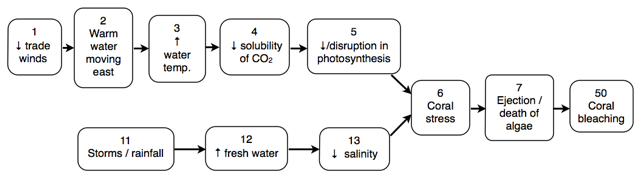
\includegraphics[height=3.6cm]{CoralBeachSemanticModel.png}
\caption{The Coral Bleaching Causal Model}
\label{fig:cb_causalmodel}
\end{figure}

Each student was provided with the essay prompt, and asked to answer the
question using the source material provided. 105 middle and high-school students
were assigned the 2 essay questions. Following completion, the essays were then
annotated by two different annotators according to how well they aligned with
the corresponding causal model. Each word was tagged with its corresponding
concept from the model, if applicable, and links were created between tagged
sequences representing the causal relationships. The inter rater reliability was
high ($\kappa$ = 0.85), and the technique proved useful in determining the level
of coherence, and the quality and completeness of the causal reasoning within
each essay.


\section{The Tagging Problem: Identifying Concept Codes}

% prior work - the concept codes were assigned only to individual sentences and
% not to the words within the sentences. Often the core concepts related to a
% few words or a phrase such as `global temps. rise' in the global warming
% essays which confounded the learning algorithm by presenting it with many
% unrelated words and phrases. In this study and prior work (peter's last paper)
% we used essays where every word was annotated to denote the corresponding
% code(s). This boosted accuracy considerably - run BOW experiment, and allows
% us to take advantage of relative positioning of words with respect to one
% another. This was not possible with annotations only on the individual
% sentences.

\section{Detecting Causality}

\section{Evaluation}
The ideal essay was one which identified all the causal concepts, and
illustrated the correct causal chains and in the correct order. To this end,
multiple metrics were defined to evaluate the relative completeness of each
student's answer compared to the causal model for the topic.
\textcolor{red}{TODO}

\section{Conclusions}

\bibliography{bib,named,apmh}
\bibliographystyle{plain}

\end{document}
